\section{Introduction}
\label{sec:intro}
With the development of globalization, mastering multiple foreign languages has become an essential skill in life and work. Fluent and accurate speaking, one of the major parts of mastering a language, will greatly improve communication efficiency\cite{ex0}. The huge demand for spoken language learning has promoted the development of computer-assisted pronunciation training(CAPT) technology~\cite{chen2016computer,fouz2015trends}. Automatic speech assessment, as one of the key technologies of CAPT, can evaluate learners' speech across various dimensions such as accuracy, fluency, and completeness. Spoken language learning is typically divided into two scenarios: the open scenario and the follow-up scenario. In the follow-up scenarios, learners are required to follow and speak out a given prompt text, while the open scenarios allow learners to express opinions freely based on a posed question. In this paper, we focus on the sentence-level pronunciation scoring of accuracy and fluency in the follow-up scenario.

% In the open scenario, require learners to express opinions freely based on a posed question, in addition to considering the aspect of speech, it will also consider the content of the speech, the accuracy and elegance of the expression, etc. The follow-up scenario is to specify a text, learners read the text, mainly focusing on the pronunciation of oral language. This paper focuses on the pronunciation scoring of accuracy and fluency at the sentence level in the follow-up scenario.
  
% 2. 目前在句子级别口语评测领域该场景下的研究可以划分为两类, 分别是align-based [5-9] 和align-free [10-12],  ASR-based相关的系统是首先给定一段语音和对应的发音文本，将发音文本和学习者的语音通过DNN-HMM的语音识别系统进行强制对齐得到音素序列、每个音素在语音片段中的起始时间和终止时间、以及从语音识别系统的声学模型中提出来的声学特征(例如隐藏层特征[9]或者通过后验概率计算的GOP特征[7])。在得到上述几种特征后，通过构建网络模型(主要部分通常为Transformer [7] 或者 BLSTM [6,8]) 将其该特征映射到对应的口语分数。另一种ASR-free相关的系统则是构建一个端到端的网络，将语音的帧级别特征和发音文本相关特征直接映射到分数，这种方法的主要是通过简化复杂的特征提取过程，排除强制对齐对打分的影响，达到简化整个打分过程的目的。在过去align-free相关[10,11,12]的系统研究中，更多的倾向于在语音的韵律相关的评估上，例如流利度打分[10,11]和韵律打分[11]，[12]主要关注于单词和音素级别的准确度打分，在关于口语的句子准确度打分上仍然存在很大的研究空间。
Most previous studies of sentence-level spoken speech evaluation fall into two categories, namely align-based~\cite{multipa,gopt,3m,our1,our2,wong22_interspeech,hipama} and align-free~\cite{liuwei,ssl1,liang23_interspeech}. Align-based systems require a DNN-HMM based Automatic speech recognition (ASR) model, which is used to perform forced alignment between the learners' speech and the corresponding prompt text. The alignment will get the phoneme sequence, the start and end times of each phoneme within the speech segment, and acoustic features extracted from the ASR system (such as hidden layer features or GOP features~\cite{gop} calculated by posterior probability). After obtaining the above features, a simple scoring network is built (usually Transformer~\cite{gopt,3m,hipama} or BLSTM~\cite{our1,our2,wong22_interspeech}) to map these features to the pronunciation scores. On the other hand, an align-free system is built with an end-to-end network, which directly maps the frame-level acoustic features and text-related features to scores. It significantly simplifies the feature extraction process and eliminates the impact of forced alignment on scoring. Past studies on align-free systems~\cite{liuwei,ssl1} have predominantly emphasized evaluating speech fluency~\cite{liuwei,ssl1} and prosody~\cite{ssl1}. In [13], the focus is on accuracy at both word and phoneme levels. Align-free system may have significant potential for sentence accuracy scoring of spoken language.
% 3. 最近, 大型语言模型(LLM)的出现表现出了强大的语言理解和生成能力，并涌现出了一些小参数模型所不具备的能力，例如指令遵循和in-context learning。先前有大量的研究[14,15,16,17]利用这种大型语言模型来实现文本相关的分数预测任务，例如approach[17] 要求 LLM 首先分析和解释所提供的材料，然后再确定最终的分数, 这种方法不仅会生成分数结果，还会对学生的答案提供详细的评论，帮助学生学习如何在下一次改进。 此外，语言模型的潜力不仅仅局限于文本任务，它能很好处理并理解音频，图像等非文本信息，从而弥合不同模态之间的差距。在语音领域, 基于语言模型的语音多模态体系结构通常由三个主要部件组成: 语音编码器、模态适合器和语言模型。基于上述结构的一些比较具有代表性的多模态模型，例如SALMONN, Qwen-Audio 和 SALM, 它们将连续语音和文本的emebdding进行结合后送入到decoder-only的语言模型中，在语音理解和识别任务上展现了强大的效果。

Recently, the emergence of large language models (LLMs) \cite{gpt4,llama,qwen} has demonstrated powerful language understanding and content generation capabilities, introducing some abilities that are not present in smaller-scale language models~\cite{llm_survey}, such as instruction following and in-context learning. Some previous research~\cite{text_score1,text_score2,text_score3,text_score4} has used LLMs to implement text-related scoring tasks. For example, the study~\cite{text_score3} asks the LLM first to analyze and interpret the provided materials, and then determine the final score. This method not only generates score results but also provides detailed comments on the student’s answers. In addition, the potential of LLM is not limited to text-related tasks. They can handle and understand non-text information such as audio and images well, thereby bridging the gap between different modalities. In the field of speech, the multi-modal models based on LLM usually consist of three main components: a speech encoder, a modality adapter, and a language model. Some representative multi-modal models~\cite{salmonn,wavllm,salm,qwen_audio}, such as SALMONN~\cite{salmonn}, Qwen-Audio~\cite{qwen_audio}, combine speech features and text embedding and feed them into a decoder-only language model, demonstrating powerful capabilities in speech understanding and recognition tasks.
% 4. 受到上面多模态模型研究和LLM在文本相关的评测任务上的积极效果的启发，在本文中我们探索了语音文本多模态模型用于口语发音评测任务，模型训练过程分为两个步骤，第一步是先训练语音识别任务，第二步是在第一步的基础上用打分数据进行微调。在打分测试阶段首先语音编码器接受学习者的语音将其编码成contextual acoustic features, 这种特征包含了口语中的韵律和内容信息，然后一个project layers将该特征映射到和语言embedding相同的空间完成模态的适配，最后将跟读文本和对应的”评测“指令embedding后与语音适配后的特征进行拼接让模型来预测该段口语的准确度分数和流利度分数。
  % 1. 据我们了解，本文是第一个使用多模态语音语言模型来对口语进行发音评测。
  % 2. 我们提出的这种多模态语言模型在第一步ASR中取得了SOTA的效果。
  % 3. 这种多模态方法没有用对齐系统，却达到了和传统系统有竞争力的性能，也验证了该方法的有效性

Inspired by the above studies on multi-modal models and the positive effects of LLMs in text-related scoring tasks, we explore the use of multi-modal models for spoken pronunciation assessment tasks in this paper. The model training process is divided into two stages. The first stage is to train the model in the speech recognition task, and then the model will be fine-tuned based on the task-specific scoring data in the second stage. When assessing a learner's speech, the speech encoder was used to map the speech into contextual features. These features contain the prosody and content information in spoken language. Then the adapter layer maps this feature to the same space as the text embedding to achieve the modality adaptation. Finally, the prompt text and the assessment task-specific prefix are embedded and concatenated with the speech features generated by the adapter layer to allow the LLM to predict the accuracy and fluency scores. The contributions of this paper are summarized as follows:


\begin{figure*}[t!]
\centering
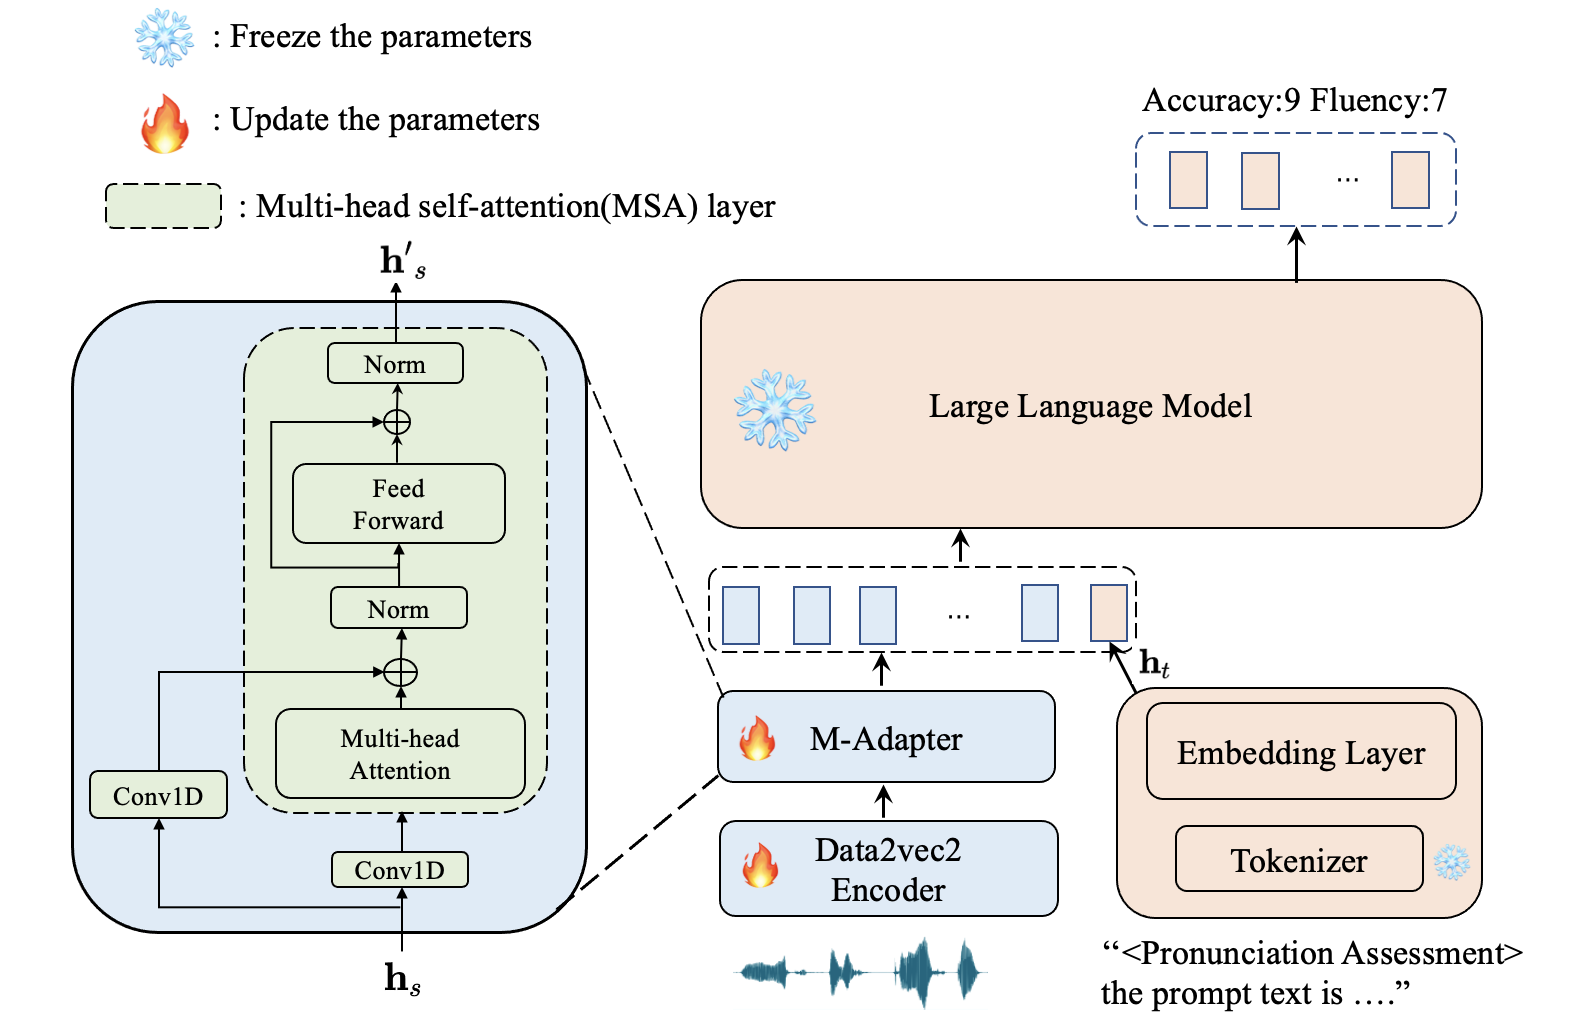
\includegraphics[width=0.6\textwidth]{content/figs/model7.png}
\caption{The overall pipeline for L2 learner's pronunciation assessment in the proposed system.}
\label{fig: model}
\end{figure*}

\begin{itemize}
    \item To our knowledge, this paper is the first to use a multi-modality model based on the LLM for pronunciation assessment. 
    \item The proposed multi-modal method belongs to the align-free system category and has achieved competitive performance compared to traditional align-based and align-free systems, which also verifies the effectiveness of this method.
    \item We contributed to a multi-modal system that achieved state-of-the-art (SOTA) results in ASR when we finished the training in the first stage.
\end{itemize}
